\documentclass{beamer}

\usepackage[russian]{babel}
\usepackage[utf8]{inputenc}
\usepackage{cmap}
\usepackage{graphicx}
\usepackage{xspace}
\usepackage{psfrag}
\usepackage{float}

\newcommand{\MARK}[1]{{\bf {\it #1}}}
\newcommand{\CODE}[1]{{\ttfamily #1}}

\setbeamertemplate{footline}[frame number]
\usecolortheme{seahorse}
\beamertemplateshadingbackground{white}{blue!3}

\begin{document}

\begin{frame}
\begin{center}
Кирюшкина Валентина\\
\vspace{1cm}
{\Large Разработка утилит для тестирования целостности репозитория пакетного менеджера Deepsolver}
\end{center}
\begin{tabbing}
\hspace{6.5cm} \= Научный руководитель\\
\> Пожидаев М. С.\\
\end{tabbing}
\end{frame}

\begin{frame}
\frametitle{Дистрибуция ПО в Linux}
\textbf{Репозиторий} - централизованное хранилище программ в сети.\\
Основное свойство репозитория - целостность.\\
Программа --- \textbf{Пакет}. Пакеты тесно связаны друг с другом.

\end{frame}

\begin{frame}
\frametitle{Deepsolver}
\textbf{Deepsolver} - система управления пакетами (пакетный менеджер) от \textit{ALT Linux}\\
Проблема: необходимо осуществлять контроль целостности репозитория \textit{Deepsolver}. 

\end{frame}

\begin{frame}
\frametitle{Цель работы}
Цель настоящей работы:\\
Создание  программного 
продукта, проверяющего целостностноть репозитория Deepsolver.

\end{frame}

\begin{frame}
\frametitle{Зависимости между пакетами}
 Пакет может предоставлять функциональность другого пакета, указывая об 
этом информацию в тэге \tetxit{provide}. \\
Так же допустимы следующие типы отношений на множестве пакетов:
\begin{itemize}
\item
\textit{Requires} : пакет требует обязательное наличие другого пакета, указанного 
по его имени или по одному из его provides.
\item
\textit{Conflicts} :
пакет запрещает наличие другого пакета, указанного по его имени или по
provides.
\item 
\textit{Obsoletes}: Пакет может указывать, что является обновлением некоторого 
множества пакетов. 
\end{itemize}

\end{frame}

\begin{frame}
\frametitle{Репозиторий пакетного менеджера Deepsolver}
\begin{itemize}
\item
В репозитории около 60 000 пакетов
\item
Каждый пакет в среднем содержит 9 require и 2 provide
\end{itemize}

Следствие: удаление и добавление пакетов с учетом зависимостей ---
нетривиальная задача.\\

Изменения отражаются в метаданных репозитория - индексе.
\end{frame}

\begin{frame}
\frametitle{Изменение индекса в Deepsolver}
Механизм обновления индекса внутри атвоматизированной части  \textit{Deepsolver}.\\

Задача механизма: обеспечение целостности при внесении изменений в индекс.\\

Для обеспечения целостности - контроль работы механизма.

\end{frame}

\begin{frame}
\frametitle{Цель работы}
\begin{itemize}
\item
Создание утилиты для проверки готового индекса.
\item
Тестирование утилит для обновления индекса.
\end{itemize}

Часть проверки:отслеживание появления
неактуальных данных, засчет которых неоправданно увеличивается размер индекса.
\end{frame}

\begin{frame}
\frametitle{Индекс репозитория Deepsolver}
\begin{itemize}
\item
Индекс хранится на ftp-сервер ALT Linux.
\item
Индекс - набор файлов с информацией о пакетах репозитория различной детализации.
\item
Свой набор файлов для каждой архитектуры.
\end{itemize}
\end{frame}

\begin{frame}
\frametitle{Условия целостности репозитория}
Под целостностью
репозитория понимается состояние, которое удовлетворяет следующим
условиям:
\begin{itemize}
\item{Для каждого \textit{require} пакета существует одноименный \textit{provide} 
другого пакета. Require, для которого это условие не выполняется
называется \textit{анметом (unmet)}. }
\item{Для каждого \textit{provide} существует одноименный \textit{require/conflict} или
он находится в директории из заранее заданного списка.Это условие 
контролирует появление избыточных \textit{provide}, засчет которых
может существенно расти размер индекса.}
\item{Для каждого \textit{conflict} пакета существует одноименный \textit{provide} 
другого пакета. Это условие не является таким строгим, как два предыдущих,
но желательно, чтобы оно выполнялось. }
\end{itemize}
\end{frame}

\begin{frame}
\frametitle{Утилита для проверки готового индекса}
\textbf{Входные данные}: индекс-файл, содержащий основной
список пакетов с информацией о 
зависимостях между ними.\\

Проверка условий целостности.\\

\textbf{Выходные данные}: Статистика о наденных ошибках.

\textbf{Результат}: Серьезные ошибки и недоточеты - индикатор некорректной работы
механизма обновления индекса.
\end{frame}

\begin{frame}
\frametitle{Структура основного модуля}

\begin{figure}
\begin{center}
\vspace{0cm}
\hspace*{-1cm} 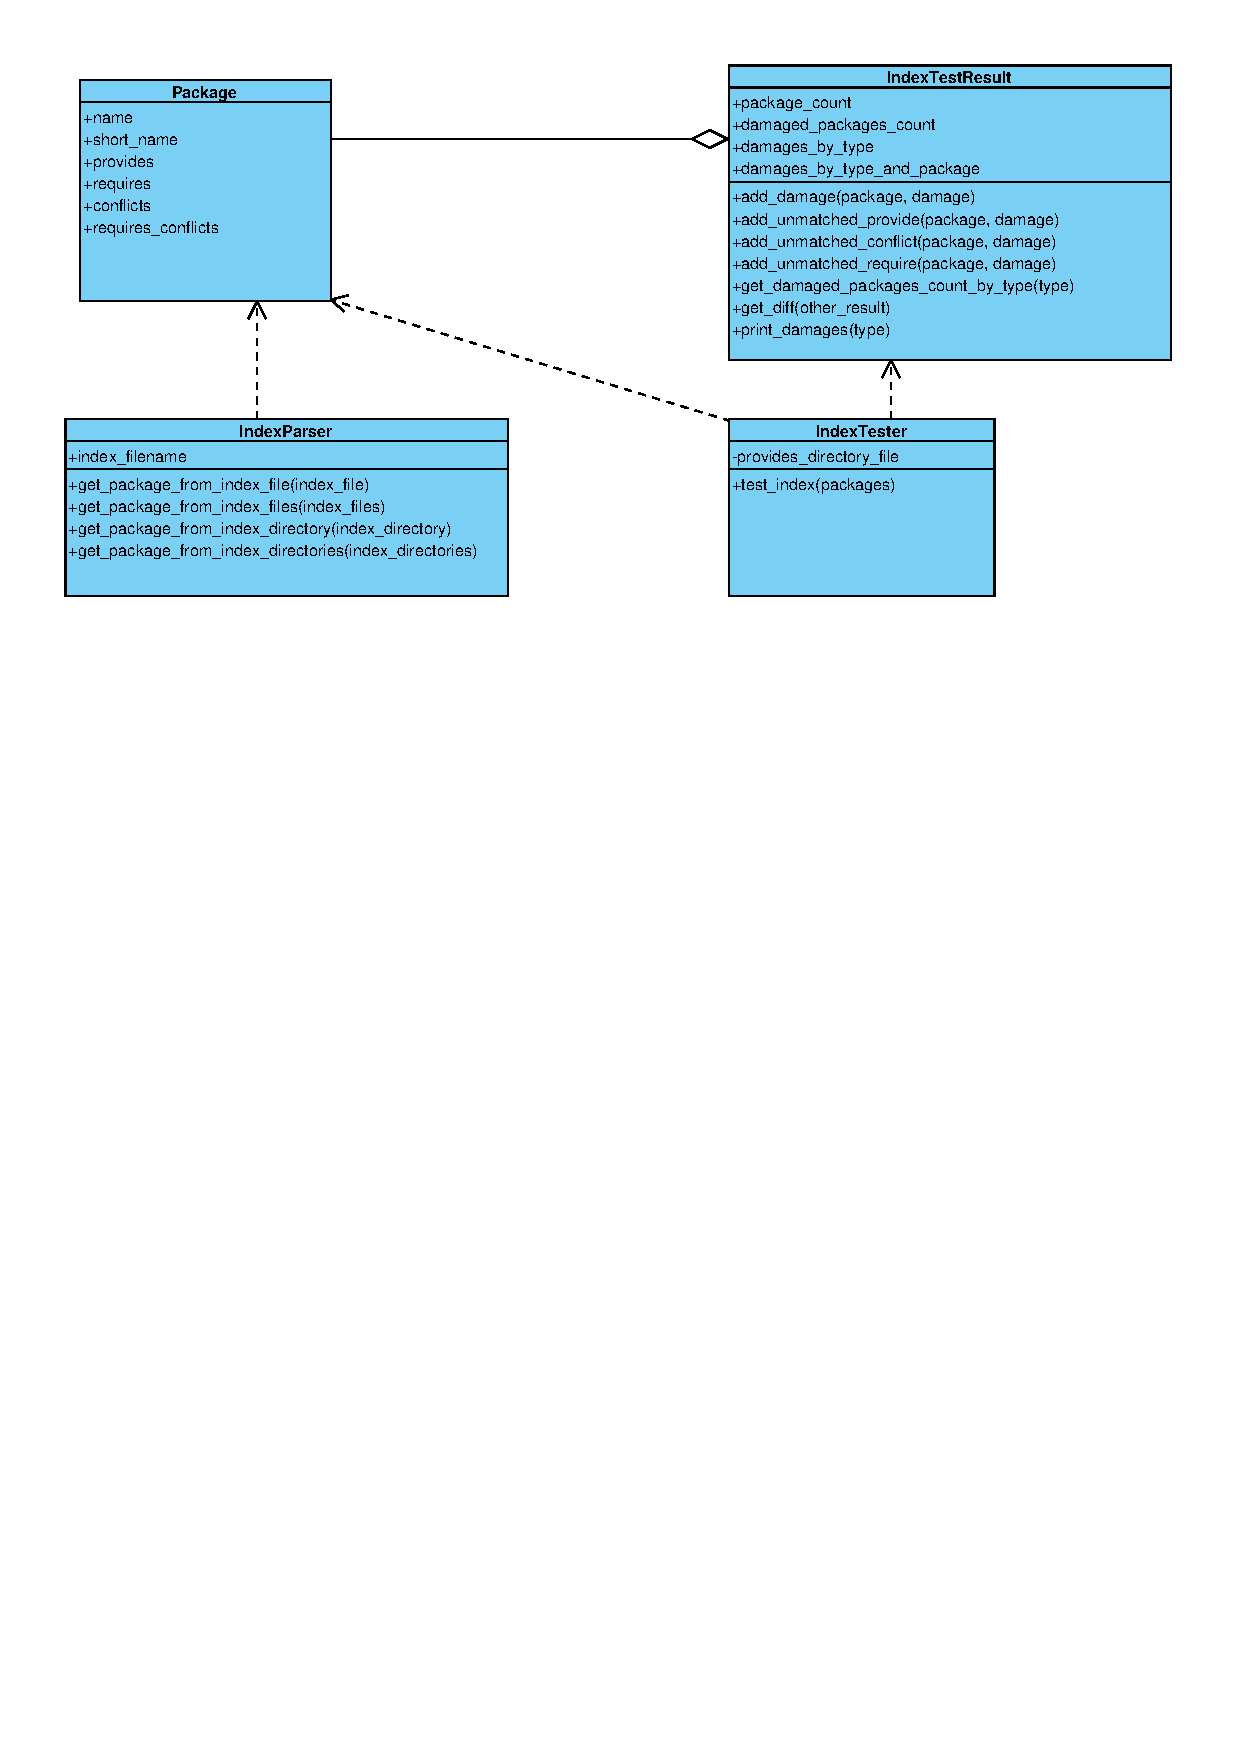
\includegraphics[scale=0.43]{../resources/uml/ds_test_class_diagram.pdf}
\end{center}
\end{figure}

\end{frame}

\begin{frame}
\frametitle{Утилита для проверки механизма обновления индекса}
Входные данные: Весь набор индекс-файлов для данной архитектуры.\\

Этапы проверки:
\begin{itemize}
\item
Проверка на неизмененнои индексе
\item
Проверка индекса после каждого запсука механизма обновления.
\end{itemize}
Выходные данные: Статистика о найденных ошибках на неизменнои индексе
и после каждого обновления.
\end{frame}

\begin{frame}
\frametitle{Результаты}
\begin{itemize}
\item
Утилита для проверки готового индекса
\item
Утилита для проверки механизма обновления индекса
\end{itemize}


Разработанный утилиты применялись для решения промышленных задач:
\begin{itemize}
\item
Активно использовались на стадии отладки процедуры обновления индекса репозитория \textit{Deepsolver}.
\item
Производилась проверка целостности индексов репозитория \textit{Deepsolver} после интеграции в официальный репозиторий
\textit{ALT Linux}.

\end{itemize}
\end{frame}

\begin{frame}
{\Large Спасибо за внимание!}
\end{frame}

\end{document}
